\documentclass[10pt]{article}


\usepackage{amsmath}
\usepackage{amssymb}
\usepackage{array}
\usepackage[english]{babel}
\usepackage{blindtext}
\usepackage{booktabs}
\usepackage{ctable}
\usepackage{enumitem}
\usepackage{fancyhdr}
\usepackage{float}
\usepackage[a4paper, margin=0.5in]{geometry}
\usepackage[utf8x]{inputenc}
\usepackage{graphicx}
\usepackage{mathrsfs}
\usepackage{placeins}
\usepackage{rotating}
\usepackage{ragged2e}
\usepackage{relsize}
\usepackage{tabularx}
\usepackage{url}
\usepackage{xcolor,colortbl}


% Quotes
\newcommand{\qn}[1]{``#1''}


\title{\textbf{An Alpha-Beta Pruning Algorithm for the Ultimate Tic-Tac-Toe Game}}
\author{Thiago V. de A. Silva\\2017719891}
\date{\today}
\begin{document}

\maketitle

\section{Introduction}

Tic-Tac-Toe is a classic 2-player game. Given a 3x3 board, the game takes place in turns, in each turn a player has to choose a blank square in the grid and put his mark on it, whoever gets three marks in a row wins. This game is extensively used as example in artificial intelligence and game theory courses. In this report, we define the player's 1 mark as X and player's 2 as O.

\begin{figure}[h]
\centering
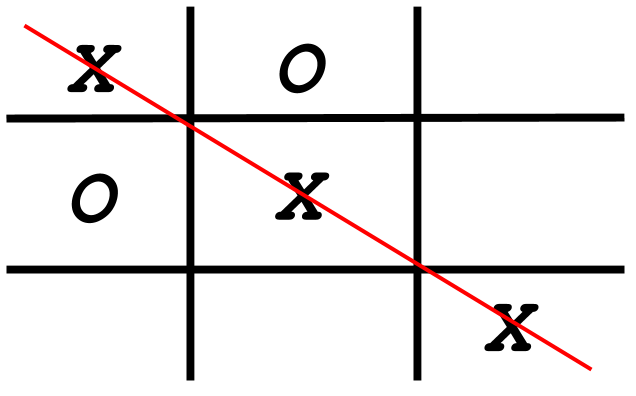
\includegraphics[scale=0.2]{img/tic-tac-toe.png}
\caption{Example of tic-tac-toe game; player 1 won!}
\end{figure}

 There are several variations of the game: 3D tic-tac-toe, Wild tic-tac-toe, Ultimate tic-tac-toe... \cite{3dtictactoe,wildtictactoe,ultimatetictactoe}. On this project, we decided to work with the ultimate version of the game. This variation is interesting because it's simple, there is no clear winning strategies, unlike the classic version, and the number of states is exponentially high.\\
 
In this work, we've implemented an alpha-beta pruning algorithm for the ultimate tic-tac-toe, and tested it considering two distinct payoff tables, and we've done a sanity test running our proposed solutions against a player that selects random positions.

\section{Game Rules}
The Ultimate tic-tac-toe is a 2-player game, just like the classic version. Given a 3x3 board, for each square there is a classic tic-tac-toe board, see the figure below for better understanding:

\begin{figure}[h]
\centering
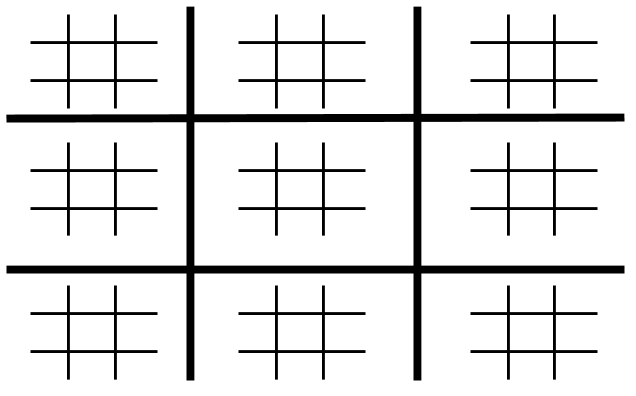
\includegraphics[scale=0.3]{img/ultimate.png}
\caption{Example of the Ultimate tic-tac-toe game}
\end{figure}

% inner and outter

The game takes place in turns: The first player starts, he chooses any inner board and put his mark in a blank square on position (i, j) of the inner game, then player 2 must play at the (i, j) board. For example: Suppose player 1 chooses the (1, 0) inner game, and marked at position (1, 2); then, player 2 must play the (1, 2) inner game next, in the figure below she played at the position (0, 0) of the (1, 2) inner board, then player 1 must play the (0, 0) inner board, and this game goes on...\\

Each play is defined by four coordinates $(x, y, i, j)$, in which $(x, y)$ indicates the outer position and $(i, j)$ indicates the inner position. Given that the first player played at $(x_1, y_1, i_1, j_1)$, for instance, then player 2 must play at $(i_1, j_1, i_2, j_2)$ next. See the example below:

\begin{figure}[h]
\centering
\begin{minipage}{.33\textwidth}
  \centering
  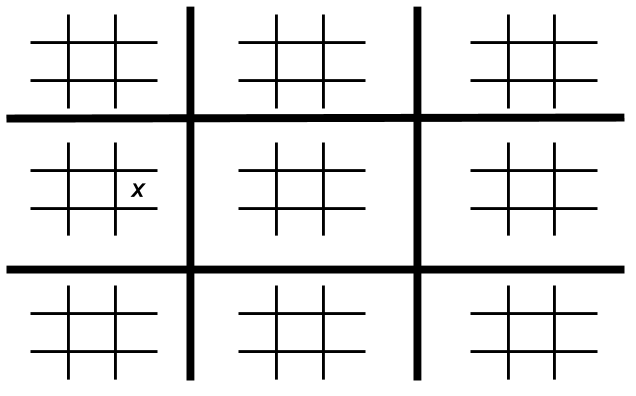
\includegraphics[width=.9\linewidth]{img/ultimate1.png}
  \caption{First turn}
\end{minipage}%
\begin{minipage}{.33\textwidth}
  \centering
  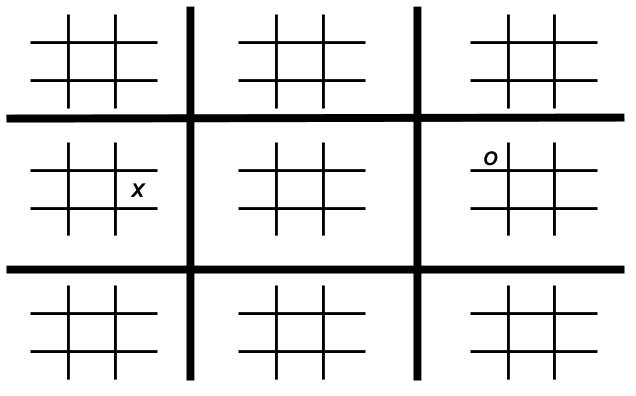
\includegraphics[width=.9\linewidth]{img/ultimate2.png}
  \caption{Second turn}
\end{minipage}
\begin{minipage}{.33\textwidth}
  \centering
  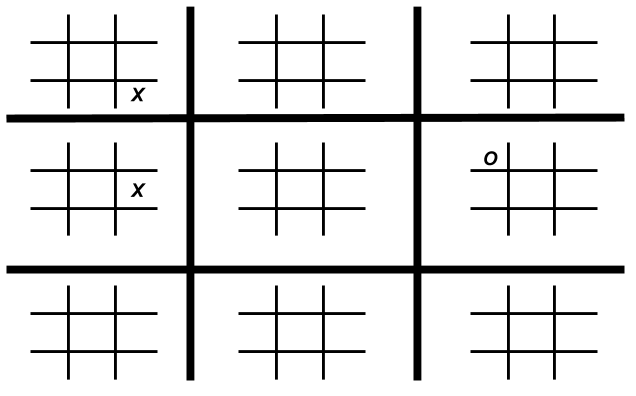
\includegraphics[width=.9\linewidth]{img/ultimate3.png}
  \caption{Third turn}
\end{minipage}
\end{figure}

In case player 2 is sent to an inner board that is already full or any player had already won that inner game, then she can play wherever she wants in the entire game.\\
If a player wins an inner game, than he gets to put a big mark on the outer position of the game he'd won. e.g.:

\begin{figure}[h]
\centering
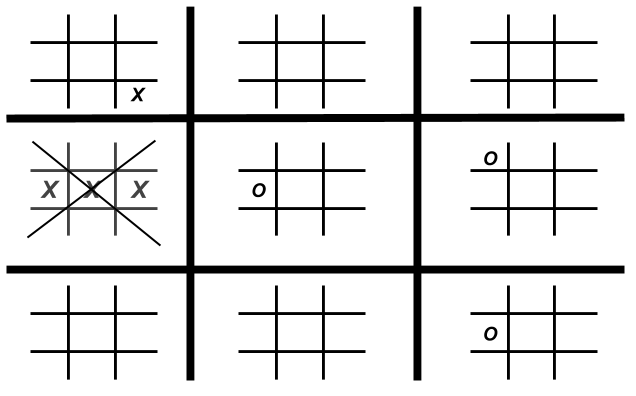
\includegraphics[scale=0.3]{img/ultimate4.png}
\end{figure}

Whoever gets three marks in a row on the outer board, wins the game.\\

\section{Payoff Tables}
We've designed two distinct payoff tables for this game, their assembling was done in order to resemble known strategies of the classic tic-tac-toe game.\\

Each strategy is defined in two parts, outer payoffs and inner payoffs. The outer payoffs corresponds to plays in which players conquers a big mark. The inner payoffs corresponds to events in which just inner boards are altered.\\

The inner payoffs are the same for all strategies: Every time a play doesn't affect the outer board, the inner payoff is set to $p = m_c - m_{opp}$, the number of marks of the current player present at the inner game minus the number of marks of the opponent.

\subsection{Conquer Center First}


\subsection{Conquer Corners First}



\section{AI}
\subsection{Random}
Talk a little bit about the random strategy.\\
Show some numbers, like the proportion of player 1 wins, proportion of player 2 wins, proportion of draws.\\
Average number of moves until the end of the game, median, standard deviation, and everything.

\subsection{Alpha-Beta Prunning}
With the first function for the $A^*$.


\section{Experiments}
\subsection{Technical Details}
Every method or algorithm described in this report was implemented in python. The whole implementation can be found in \url{https://github.com/thiagovas/Ultimate-Tic-Tac-Toe}.\\
All experiments were executed in a Intel$^\copyright$ Core {\tiny\texttrademark} 2 Duo CPU E7500 with 2 cores of 2.93GHz, and with 4Gb of RAM.
\subsection{Sanity Test}
(1) Show the experiments comparing the results

\subsection{CCeF vs CCoF}



\section{Future Work}
(1) For now, there is just the monte carlo tree search.\\
(2) Maybe create more payoff tables.\\
(3) Consider using cython, or any optimizer, given that I used python, and used it for simplicity.\\
(4) Make some pruning using the equivalent classes from that nice paper.


\section{Conclusion}



\bibliography{report}{}
\bibliographystyle{plain}

\end{document}